\documentclass[main.tex]{subfiles}
\begin{document}
\section{Background}
\label{section:background}

\subsection{Feature-Equivalent Micro-Blogging Application (MiniTwit)}

The micro-blogging application we use as the software to measure the energy consumption (in Joules) is a minimal implementation of X (formerly known as Twitter \cite{verge-twitter-rebrand-x}) called MiniTwit. Armin Ronacher initially implemented MiniTwit as an example showcasing the Python web application framework Flask \cite{ronacher-minitwit-commit}. This implementation of MiniTwit was picked up by the subject "DevOps, Software Evolution and Software Maintenance" at the IT University of Copenhagen \cite{devops-course}, as the application students have to develop and maintain during a semester. Students can either update the Flask implementation to a newer version of Python or re-implement it in another programming language and web framework. It is still required to adhere to the same set of functional requirements in either case. This results in the DevOps course gradually accumulating a set of feature-equivalent MiniTwit applications, implemented in different languages and web frameworks.

\subsection{Optimizations for Web Applications}

When researching optimization strategies for a web application, we examine some of the improvements implemented by the most popular web applications. One example is Shopify, which describes itself as "The all-in-one commerce platform to start, run, and grow a business." \cite[see the first paragraph]{shopify-about-page}. Shopify is built using Ruby on Rails \cite{shopify-yjit}, and has allocated resources to enhance the Just-In-Time (JIT) compiler in CRuby. Their new implementation, called Yet Another Ruby JIT (YJIT), was accepted into the open-source implementation of CRuby and merged upstream \cite{shopify-yjit}.

This addition has sparked renewed interest from Ruby developers, who have subsequently tested whether their applications would benefit from using YJIT. An example is Matt Haliski, who upgraded his website to use YJIT and jemalloc, and found a drop in memory use ($\approx 250 mb$) \cite{matt-haliski-yjit-jemalloc-upgarde}.

The change of memory allocator to jemalloc is another optimization we see in other web applications. Facebook hired the creator of the memory allocator, jemalloc, to resolve scaling issues with \cite{facebook-jemalloc} and saw a significant performance increase by using jemalloc over malloc.

Another optimization technique similar to JIT is Profile-Guided Optimization (PGO). PGO analyzes the usage patterns of an application and performs optimizations based on this data. This paper uses Feedback-Directed Optimization (FDO) as a shared term for JIT compilation and PGO, although historically, FDO and PGO were used interchangeably \cite{Wicht_Vitillo_Chen_Levinthal_2014}.

\subsubsection{Profile Guided Optimizations (PGO)}

Performing PGO involves two main steps. First, usage data must be collected from the application while running with a real-life workload. Second, this usage data guides specific optimizations, such as embedding smaller functions into larger ones, when the application is recompiled \cite{Wade_Kulkarni_Jantz_2017}.

Because usage data must be collected before optimizations can be performed, PGO is static and cannot adapt to changes in usage patterns without human intervention \cite{Wade_Kulkarni_Jantz_2017}. 

\subsubsection{Just-In-Time (JIT) Compilations}

Just-In-Time (JIT) compilation applies the same optimizations as PGO \cite{Wade_Kulkarni_Jantz_2017}, but dynamically. It can collect usage data, analyze it, identify optimizations, and apply them at runtime without requiring the application to be rebuilt.

How JIT precisely works depends on the specific implementation. Generally, when an interpreter compiles the code to machine code, it optimizes according to the latest collected usage data \cite{Wade_Kulkarni_Jantz_2017}. 

Applying optimizations at runtime, JIT introduces overhead compared to PGO. The collection and analysis of usage data, combined with code optimizations, affect the program's runtime and can cause an initial performance hit \cite{Aycock_2003}.

 \subsection{Memory Allocators}

The responsibility of a memory allocator is to handle the allocation and deallocation of memory. The C standard library (libc) \cite{c-language-iso9899-2024} exposes a set of functions to manage memory, known as malloc. Libc allows the developers to implement these memory functions, thereby allowing multiple versions of malloc \cite{Berger_Zorn_McKinley}.  The two malloc implementations relevant to this paper are the malloc implementation provided via the glibc library \cite{glibc} and jemalloc \cite{evans2006scalable}.

\subsubsection{jemalloc}
malloc is generally effective for most applications. However, it can struggle in highly concurrent and multithreaded environments, such as web applications \cite{evans2006scalable}. 

To address these challenges, Jason Evans developed a custom memory allocator called jemalloc \cite{evans2006scalable}. One issue with malloc in a multithreaded context is that each thread must acquire a lock to manage memory, which can lead to performance bottlenecks. jemalloc would resolve this by splitting memory into arenas (see figure \ref{fig:malloc-vs-jemalloc}).

The use of arenas mitigates the lock contention issue of malloc. Each thread only has to compete for the memory lock with threads within the same arena, which is a subset of the total number of threads. The drawbacks of using arenas are the relative fragmentation they cause to memory and the overhead of managing the arenas \cite{evans2006scalable}.

\begin{figure}[h]
    \centering
    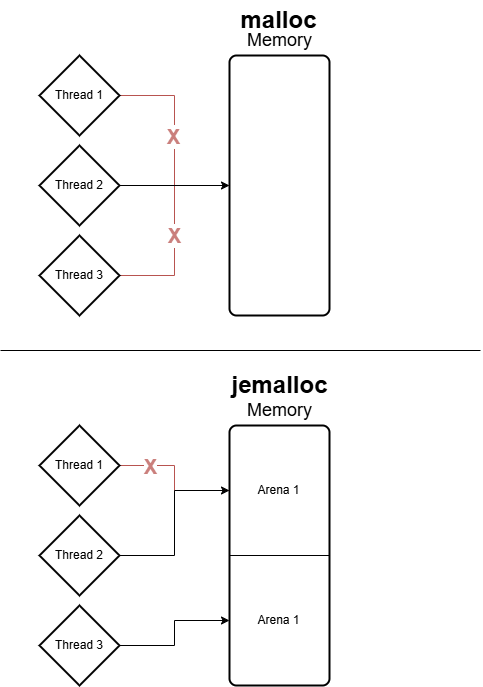
\includegraphics[width=0.8\columnwidth]{media/background/experiment-jemalloc-arenas.drawio.png}
    \caption{Visual comparison between jemalloc and malloc}
    \label{fig:malloc-vs-jemalloc}
\end{figure}

\subsection{Temperature}
According to the equation $P=I^2 \times R$ , the power draw (in Watts) increases as the resistance goes up. The resistance increases at higher temperatures in conductive materials \cite{ling2016university}. Transistors may leak current, and devices may throttle due to higher temperatures \cite{benoit2020impact}.  
\end{document}
